\chapter{Architectural Design}

\section{Overview}
The architecture that was chosen for our application is the three-tier one, because we think that this division is the most natural to represent it and is composed of: 
\begin{itemize}
	\item \textbf{Presentation tier}: contains the user interface and the communication layer of the application. Its main purpose is to display information and 			collect information from the user.

	\item \textbf{Application tier}: is the core of the application. In this tier, information collected in the presentation tier is processed, sometimes against 			other information in the data tier to offer the different functionality and services.

	\item \textbf{Data tier}: is the tier that contains the database, and so its job is to store persistently and manage data processed by the application tier and 	make it available back at the application tier.
\end{itemize}
Since the application interface is light and does not require too much computational power to work.
Instead the main services offered by our application requires the coordination of all clients a to manage the queue in real time and requires the elaboration of their real time data, and server data to predict their behavior. It needs so a central component that has a high computational power to manage it and the logic tier describes it perfectly. The application needs to record a lot of data about the customers and so a data tier is required, this data will not only be collected by the application, but it will be also collected from the supermarket chain database.
We chose the three-tier architecture also for its properties that are:
\begin{itemize}
	\item \textbf{Scalability}: any tier can be scaled independently as needed without affecting the others.

	\item \textbf{Security}: since the presentation tier and the data tier are not directly connected, it is possible to implement firewalls preventing different 			kind of unwanted exploits

	\item \textbf{Maintainability}: since the three tiers works independently from each other, updates and maintenance can be done one tier at time without 			affecting the others and by only one team. 
\end{itemize}
In our case the three tiers will contain the following division:
\begin{itemize}
	\item \textbf{Presentation tier}: will contain the interfaces showed in the mock-ups, and it will allow the users to send request for creating, deleting, and viewing line-up and booking ticket from them application. It will allow the physical spot to create and print the line-up ticket. It will allow the manager to do query on different kind of data and to interact with the realizing of new ticket and people entrances. 

	\item \textbf{Application tier}: will contain the function to manage in real time the queue considering the realizing time of the different kind of tickets, the position of the application-users, the presence of booking tickets. It will also contain the function to handle and to redirect the different kinds of the request on the appropriate component. And also, the function to check the QR code and allow user to enter, the function to build the visual representation of manager query, and the sign-up and login services.

	\item \textbf{Data tier}: will contain the information about the users, their behavior ( tendency to arrive later or early, typical staying time, etc) and all information that could help to improve the accuracy of predictions.
\end{itemize}

\begin{figure}[H]
	\centering
	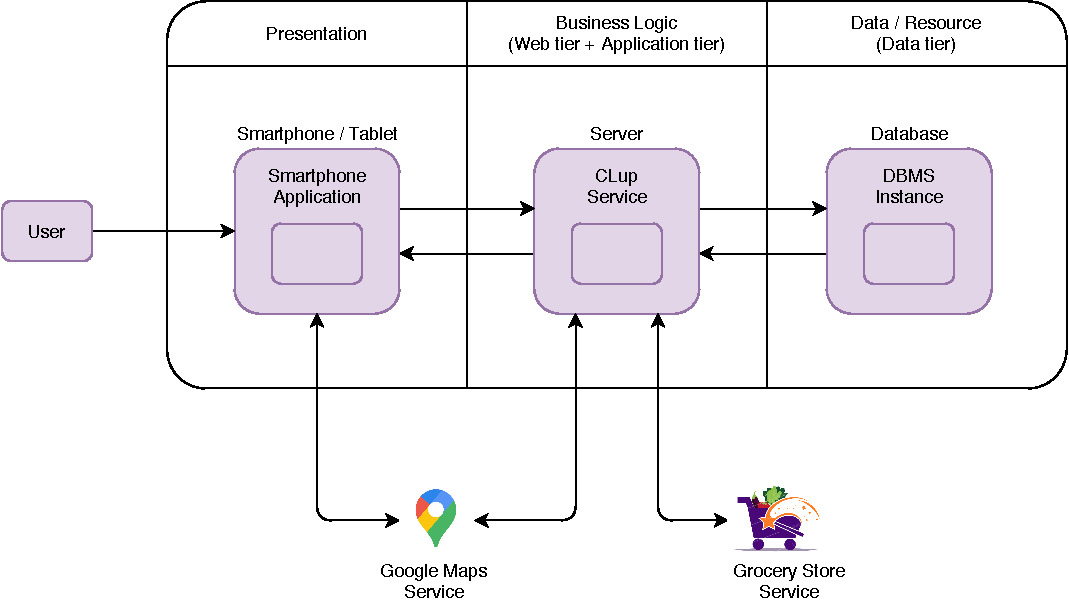
\includegraphics[width=1.0\textwidth]{images/architecture.pdf}
	\caption{System architecture.}
\end{figure}

\section{Component View}

The previously introduced components will be presented in details in this section by using the component diagram~\ref{fig:ComponentDiagram} that has been divided in three main sub-components to better understand the relation between the three tiers of the system.

The presentation tier has been represented by the \textbf{EndUserApp} that generalizes the architecture of the smartphone application.
It encapsulates the \textbf{\gls{mvc}}, that has been chosen as design pattern, and the \textbf{HostService} which is the module that allows the application to use the \glspl{api} offered by the device.

\begin{sidewaystable} % \begin{figure}[H]
	\centering
	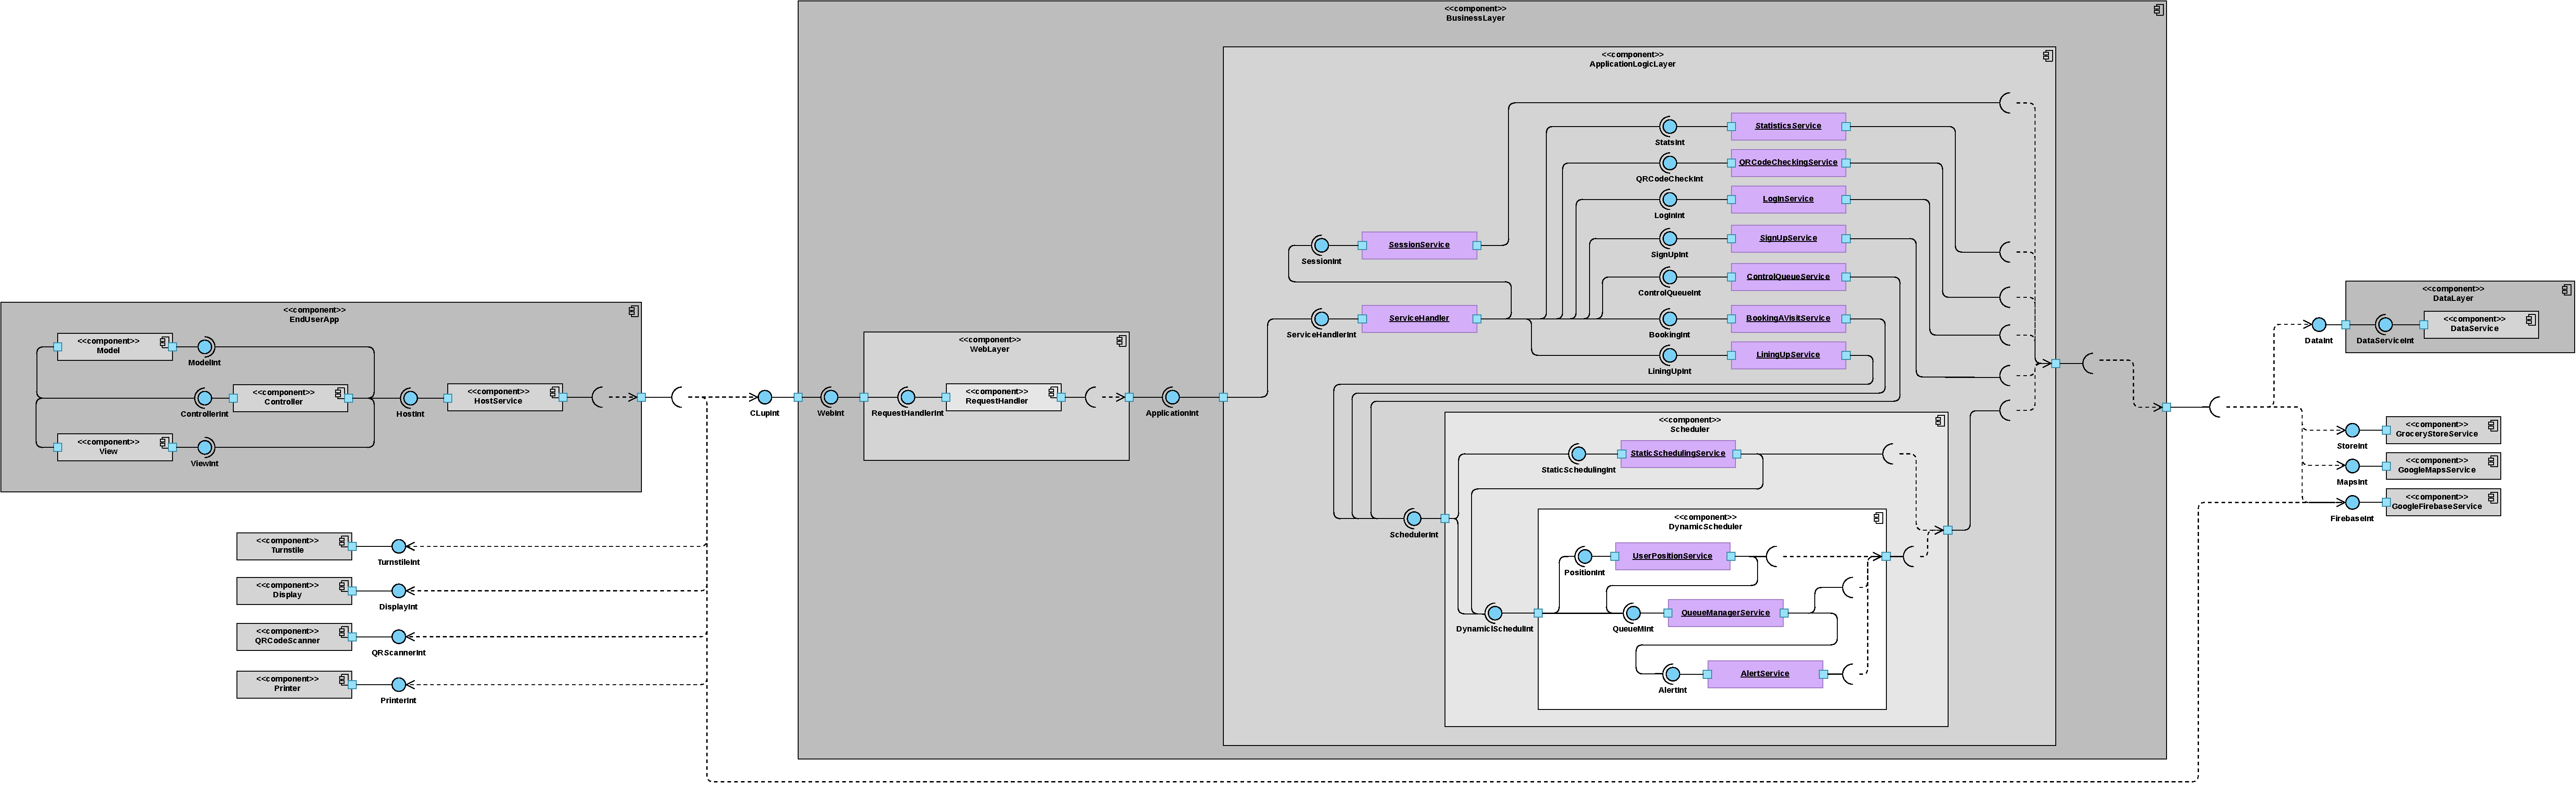
\includegraphics[width=1.0\textwidth]{images/component_diagram.pdf}
	\caption{Component Diagram.}\label{fig:ComponentDiagram}
\end{sidewaystable} % \end{figure}

The business tier (web tier \& application tier) is the most complex part of the diagram, therefore it has been split in different layers of components:
\begin{itemize}
	\item \textbf{WebLayer}: contains the \textbf{RequestHandler} component that receives the requests from remote devices and forwards them to the application tier. The main functionalities are: \textit{decryption}, \textit{parsing} and \textit{forwarding} of the requests; \textit{reformatting} (in \gls{json} format) and \textit{encryption} of the responses before sending them to the clients.
	
	\item \textbf{ApplicationLogicLayer}: contains the modules for the functionalities offered by the system. They are:
		\begin{itemize}
			\item \textbf{ServiceHandler}: is the module that coordinates the others. It receives the requests from the previous layer and checks if sessions are active, communicating with the SessionService. After that, it calls the other services based on the request type. In the end, it returns the responses to the WebLayer.
			\item \textbf{SessionService}: is the service that monitors the session by updating and releasing tokens.
			\item \textbf{StatisticsService}: is the service that creates charts for the store manager to analyze the trend of the queues. It interacts with the DataLayer to retrieve data from the database.
			\item \textbf{QRCodeCheckingService}: is the service used when customers scan the QR codes to verify that the ticket numbers are the same that have been notified by the system. It is called, in background, by the application running on the store manager device.
			\item \textbf{LogInService}: is the service that controls and updates the status of the tokens. If an user has been recognized, by the system, it changes the status of the token in the database. In this way, the user will be identified as logged and he will be able to request for services that requires an authentication.
			This service is used for log out too.
			\item \textbf{SignUpSerivice}: allows users to create an account.
			\item \textbf{ControlQueueService}: is the service used by the store manager to change parameters that modify the sequence of events in the Scheduler. From this service the store manager can modify the timing in which tickets are released, he can interrupt the release of tickets and he can change other parameters of the scheduler algorithm. This service communicates with the Scheduler and the DataLayer to store the new parameters.
			\item \textbf{BookingAVisitService}: is the service that allows customers to book a visit. It handles the data passed from the clients, performs some checks on the inserted information and communicates with the Scheduler and with the DataLayer.
			\item \textbf{LiningUpService}: is the service that allows customers to line up. As for the BookingAVisitService, it passes data to the Scheduler and the DataLayer.
		\end{itemize}
		
		The main core of the ApplicationLogicLayer is the \textbf{Scheduler} that implements the algorithm used by the system to create and keep updated the virtual queue of users. It is composed by a StaticSchedulingService and a DynamicScheduler.
		\item The \textbf{StaticSchedulingService} is in charge of performing few checks before asking to the DynamicScheduler to insert customers in the queue. Moreover, it is the first sub-module to be called by the LiningUpService and the BookingAVisitService. It communicates with the external services to compute a raw estimation of the time in which a customer will be called by the system to be authorized to enter in the store.
		\item The \textbf{DynamicScheduler} is composed by different sub-services that are necessary to update the virtual queue in background and to notify customers.
		The main sub-service is the \textbf{QueueManagerService} that handles the queue and coordinates the other modules.
\end{itemize}

The data tier has been represented by the \textbf{DataLayer} that contains the \textbf{DataService}. It interacts with the \gls{dbms} to execute queries.

In the diagram has been reported the external services used by the system:
\begin{itemize}
	\item \textbf{GroceryStoreService}: to obtain data about customers from the store.
	\item \textbf{GoogleMapsService}: used to compute the estimated time to arrive to the store from the location of the customer.
	\item \textbf{GoogleFirebaseService}: used to notify customers.
\end{itemize}


\section{Deployment View}
\begin{itemize}
	\item \textbf{Presentation tier:}In this tier we have the interfaces for the different users, the application contains all the interfaces and when the user log in the interfaces change to the proper one. For the customers, the interface permits the user to connect to the BookAVisitService, LiningUpService and ControlQueueService. In a similar way the physical spot interface permits it to connect to the Lining up service and to the feature to print. And for the manager the interface, it permits him to connect and use StaticsService, QRCodeCheckingService and ControlQueueService.

	\item \textbf{Application tier:}: In this tier we have the application server that manages all the functions of Clup. Starting from handling all the user request and redirect them to the right service required, to sending request to database to retrieve and record data. Inside this server the function the require more resources are the handling of the request and the scheduling service. Since it requires to schedule first the different kind of user and then if possible, monitor their position in line and compute it to their records of past visit.

	\item \textbf{Data tier:}In this tier the data service handles all the request coming from the application tier. It schedules the different request of transaction from the different services and manages it accordingly. So, it let them store, manage and query data of the Database. The model of DBMS used in this application is the relational one since it is the most well-known and used one. Therefore, there are a lot of tools and \glspl{api} up to date to support the work. It also fits the application requirements since it permits to compute quickly complex queries and help the data organise in a well-structured way. The first especially is needed for the scheduler, since it has to re-compute the data a lot of times during a day. 
\end{itemize}
In the application tier we have two main device that can contain the application, in particular the smartphone is associated to customers and the tablet to the physical spot and the store manager. The smartphone application also interacts via Google \gls{api} with Google Firebase Service to receive the notifications from the system. The application of both the devices can connect to the application server, which must first pass through a firewall, to increase the security of the system and then through a load balancer to distribute the workload. 
The application server is connected to both Google services also through a firewall to retrieve the position of the user in line and to send notifications. It is connected to the grocery store service to retrieve information about user’s behavior. And it is connected to also to \gls{clup} database to retrieve stats, queue information, reservation, etc. 

\begin{figure}[H]
	\centering
	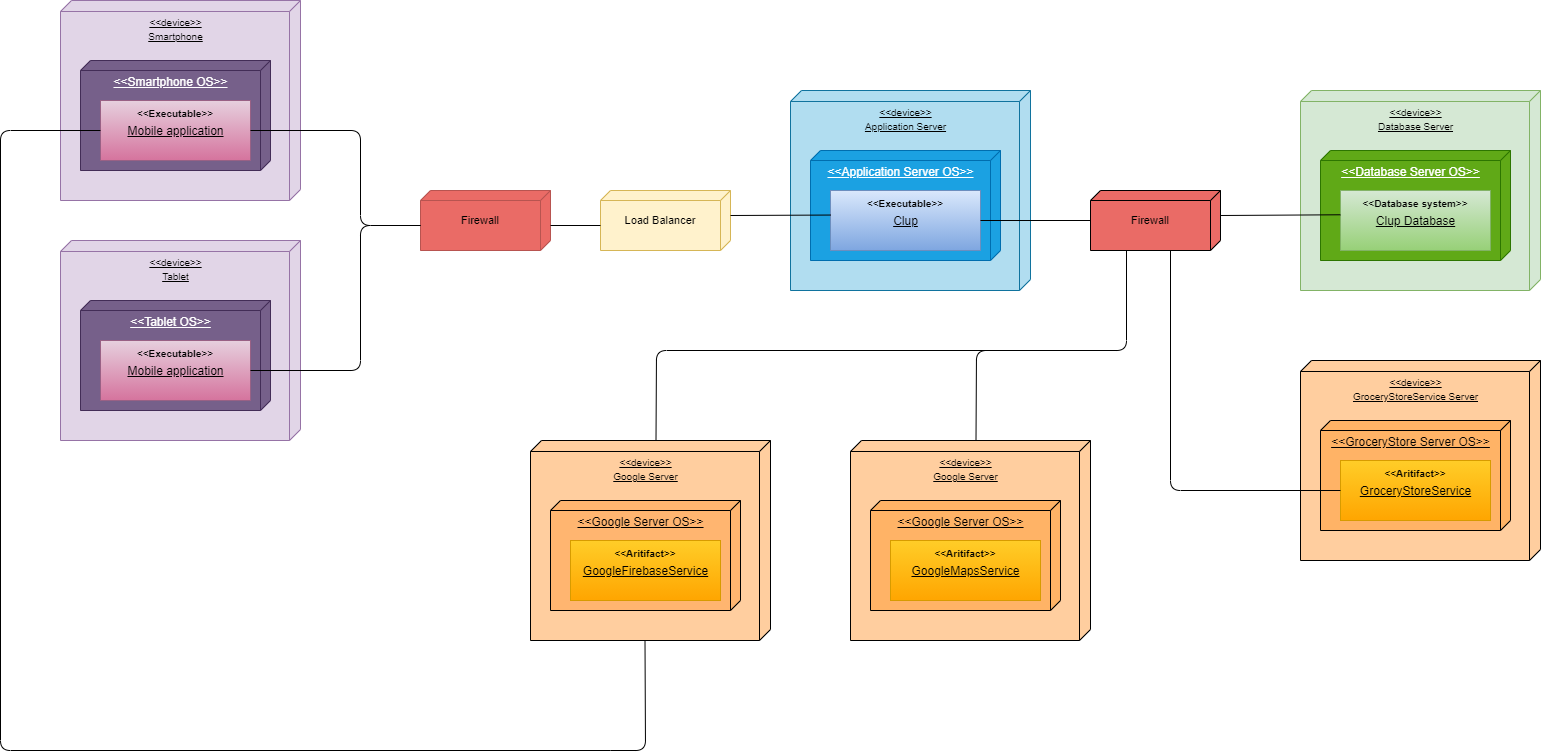
\includegraphics[width=1.0\textwidth]{images/deployment_view.png}
	\caption{Deployment diagram}\label{fig:Deployment diagram}
\end{figure}

\section{Runtime View}

In this section we are going to present how the components interact at runtime.

\subsection{Session Control}

The figure \footnote{For all the sequence diagrams, a custom notation has been used to show the input parameters of the methods (**data). It follows a programming language notation to represent inputs in a more compact way. In Python style, it can be interpreted as a dictionary data structure.}~\ref{fig:SessControl} shows the sequence diagram associated to the operations performed by the SessionService module to generate and to control the validity of a given token. The tokens are part of the request parameters, they are used to keep sessions alive with users. The SessionService checks if a token already exists; if it is, then the module controls if it is valid or expired, otherwise it will generate a new one.
Authentications and tokens are two different things: an user can have a token but he might be unauthorized (not logged or he could not have an account yet). The authorization status, associated to a token, will be updated by the LogInService or by activities performed in background by the system.

\begin{figure}[H]
	\centering
	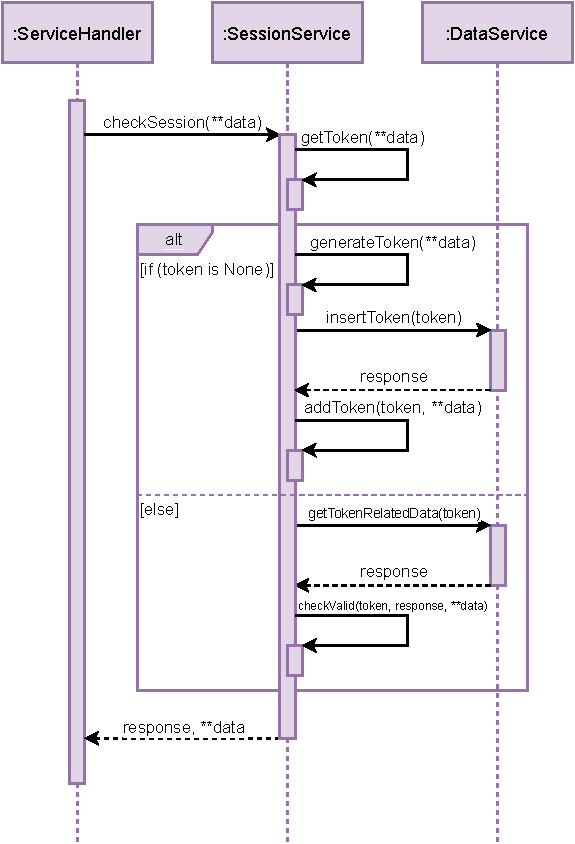
\includegraphics[width=1.0\textwidth]{images/sessionToken_sequence_diagram.pdf}
	\caption{Session control sequence diagram.}\label{fig:SessControl}
\end{figure}

\subsection{Sign Up}

In figure~\ref{fig:SignUp} has been shown the procedure to register a new user. The core of the sequence diagram is the SignUpService that filters the data inserted by the customers and controls if the credentials have already been used for other accounts. If possible, the service creates the new account by inserting the credentials, and the other customers information, in the database. Results of the queries and the other executed methods are appended to the data that are back-propagated to the RequestHandler that creates the \gls{json} response.

\begin{figure}[H]
	\centering
	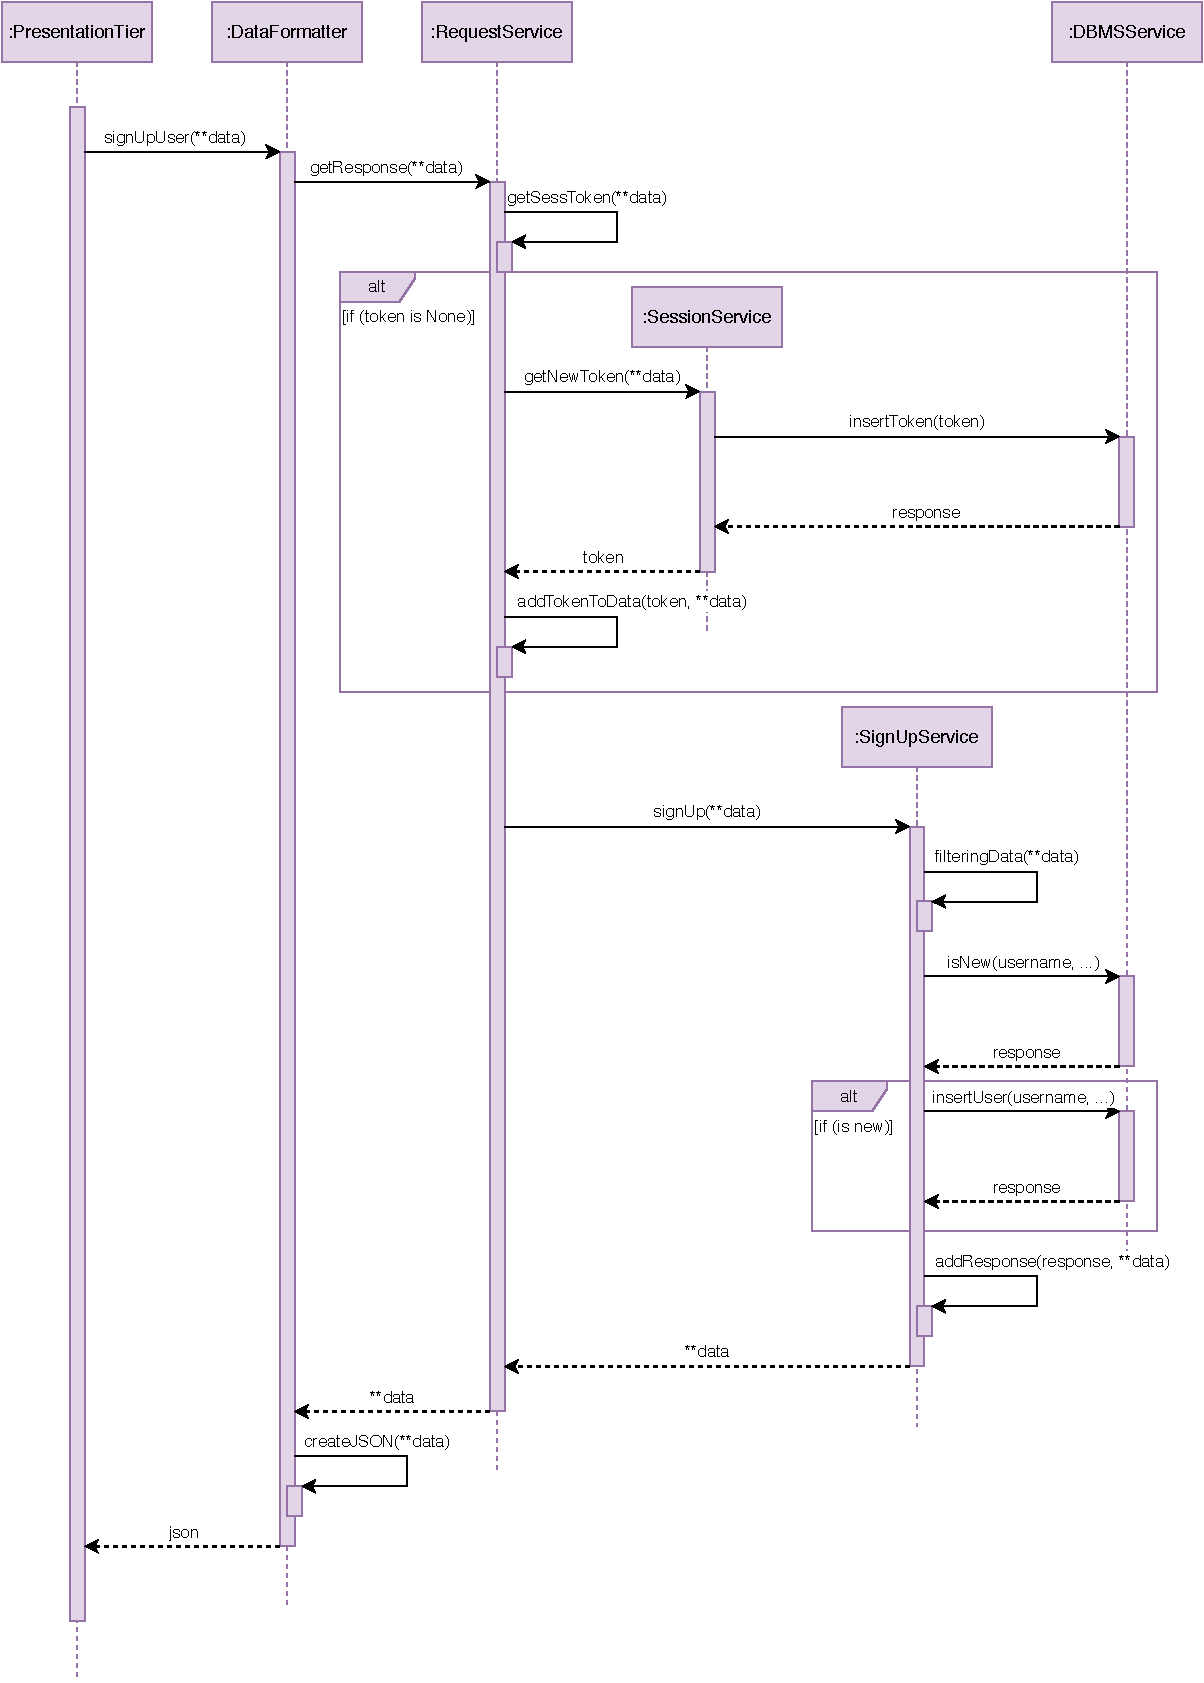
\includegraphics[width=1.0\textwidth]{images/signUp_sequence_diagram.pdf}
	\caption{Sign Up sequence diagram.}\label{fig:SignUp}
\end{figure}

\subsection{Log In}

Similarly to the sign up, the figure~\ref{fig:LogIn} shows how the log in is performed. In this case the credentials are parsed from the request parameters and a verification is performed. If the pair username-password is present in the database, then the status of the token, assigned to the customer, will be updated to remember that the user has been authenticated.

\begin{figure}[H]
	\centering
	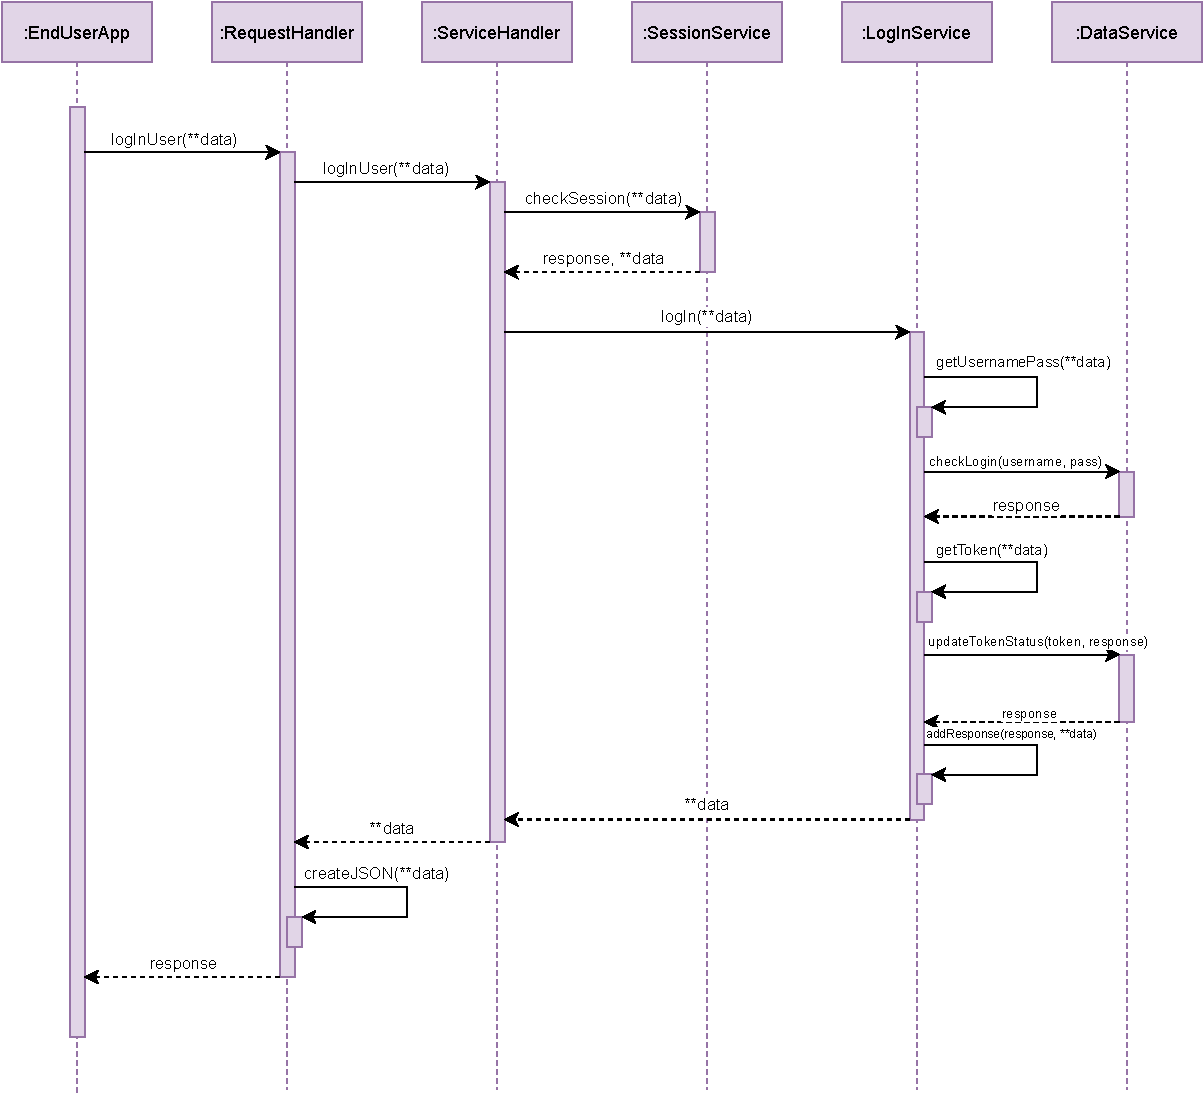
\includegraphics[width=1.0\textwidth]{images/logIn_sequence_diagram.pdf}
	\caption{Log In sequence diagram.}\label{fig:LogIn}
\end{figure}

\subsection{Lining Up}

In figure~\ref{fig:LiningUp} the lining up operation has been reported.
The user, to be allowed to perform a lining up, has to be registered and authenticated, therefore the ServiceHandler checks the token validity, communicating with the SessionService, and controls if the user is authenticated by getting the status of the token from the DataService.
In case of valid token with positive status (user before logged in), the request is forwarded to the LiningUpService, which after few controls, can decide to pass the lining up information to the Scheduler.
In any case the RequestHandler will reply to the clients with a response that it will contain lining up information (such as the QR code) or an error message.

\begin{figure}[H]
	\centering
	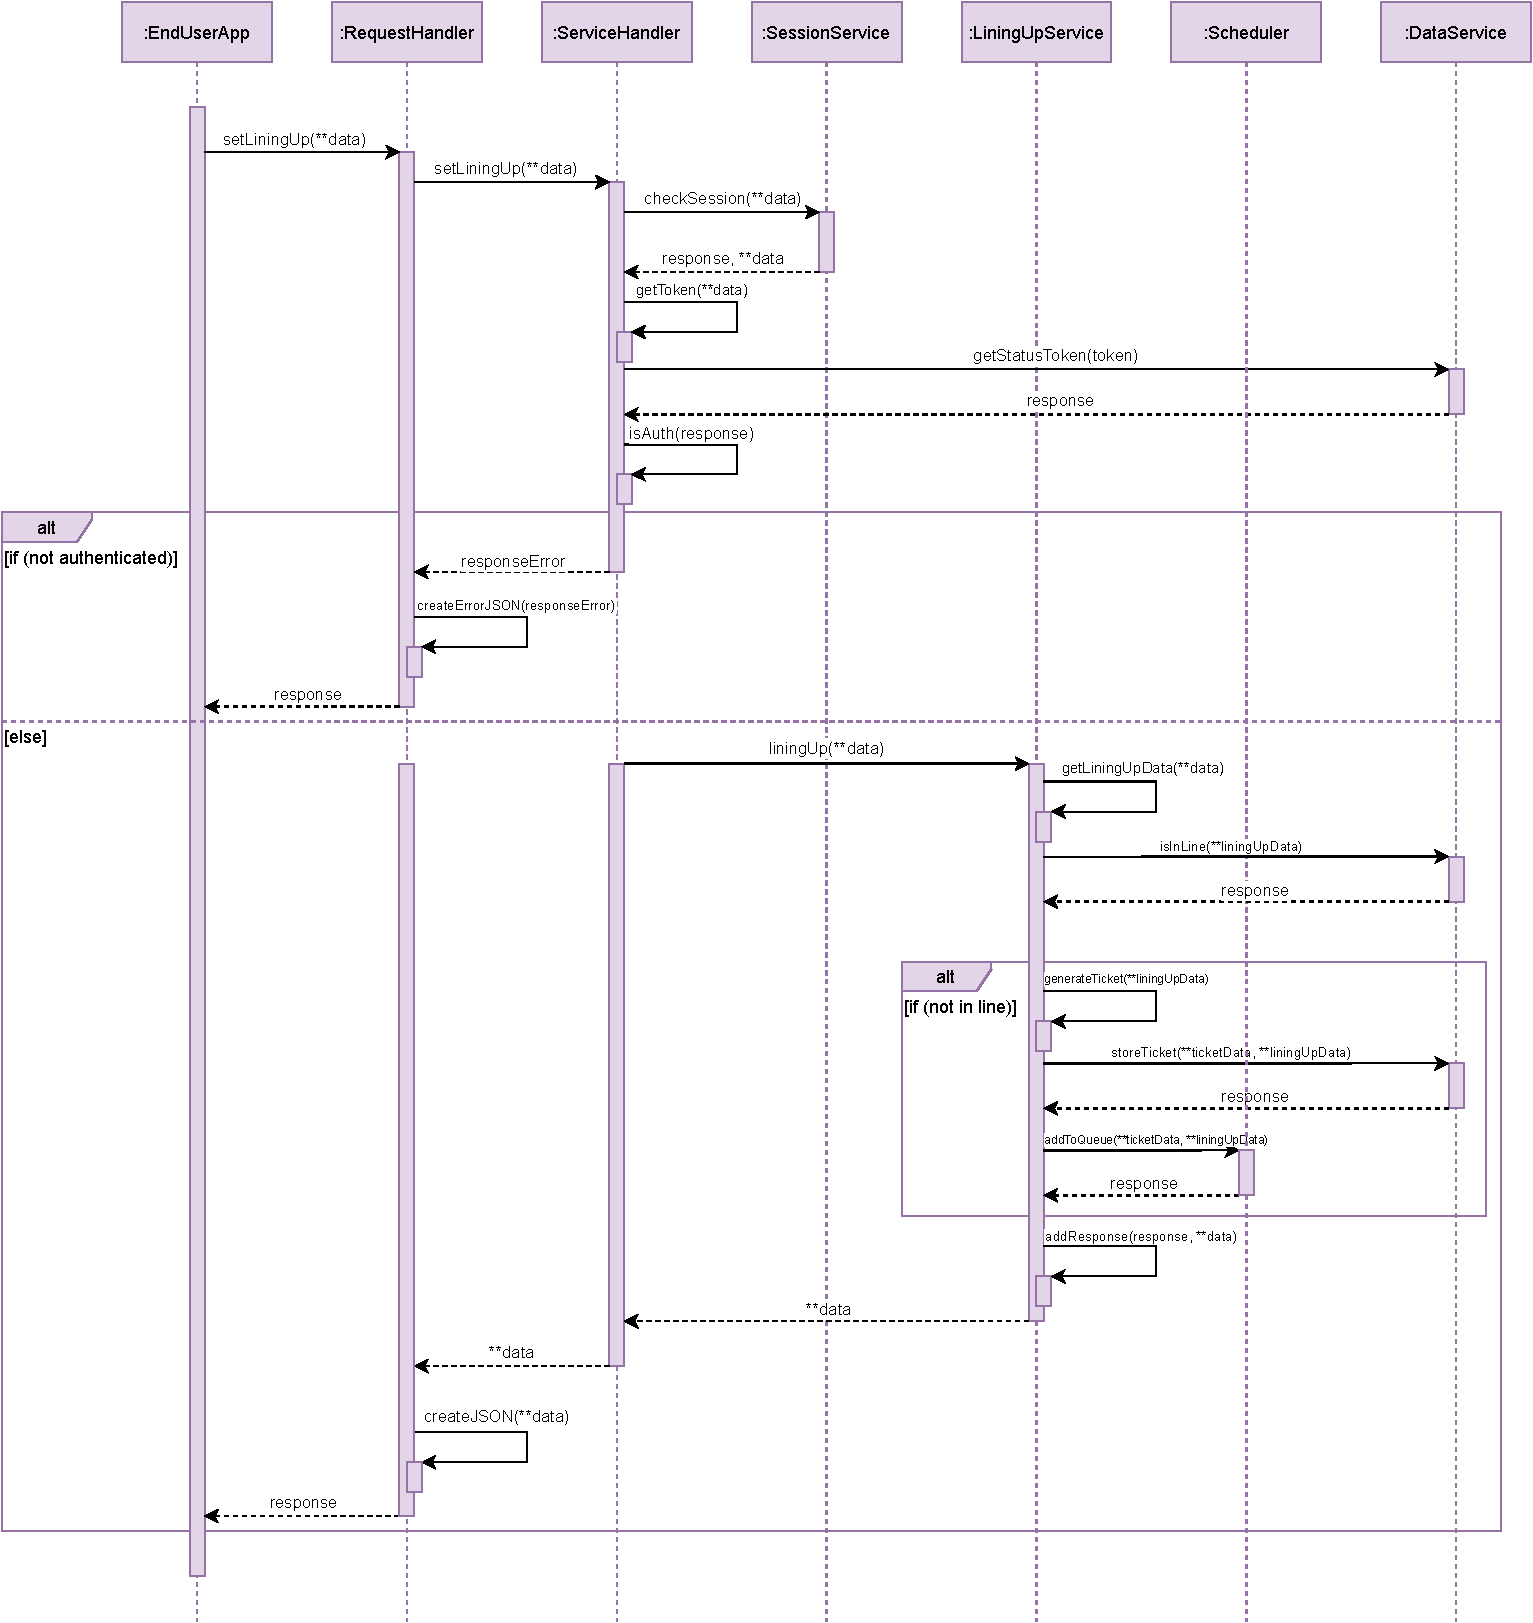
\includegraphics[width=1.0\textwidth]{images/liningUp_sequence_diagram.pdf}
	\caption{Lining Up sequence diagram.}\label{fig:LiningUp}
\end{figure}

\subsection{Booking a Visit}

The sequence diagram~\ref{fig:BookingVisit} is similar to the previous one.
The differences are in the kind of information passed from the EndUserApp.

\begin{figure}[H]
	\centering
	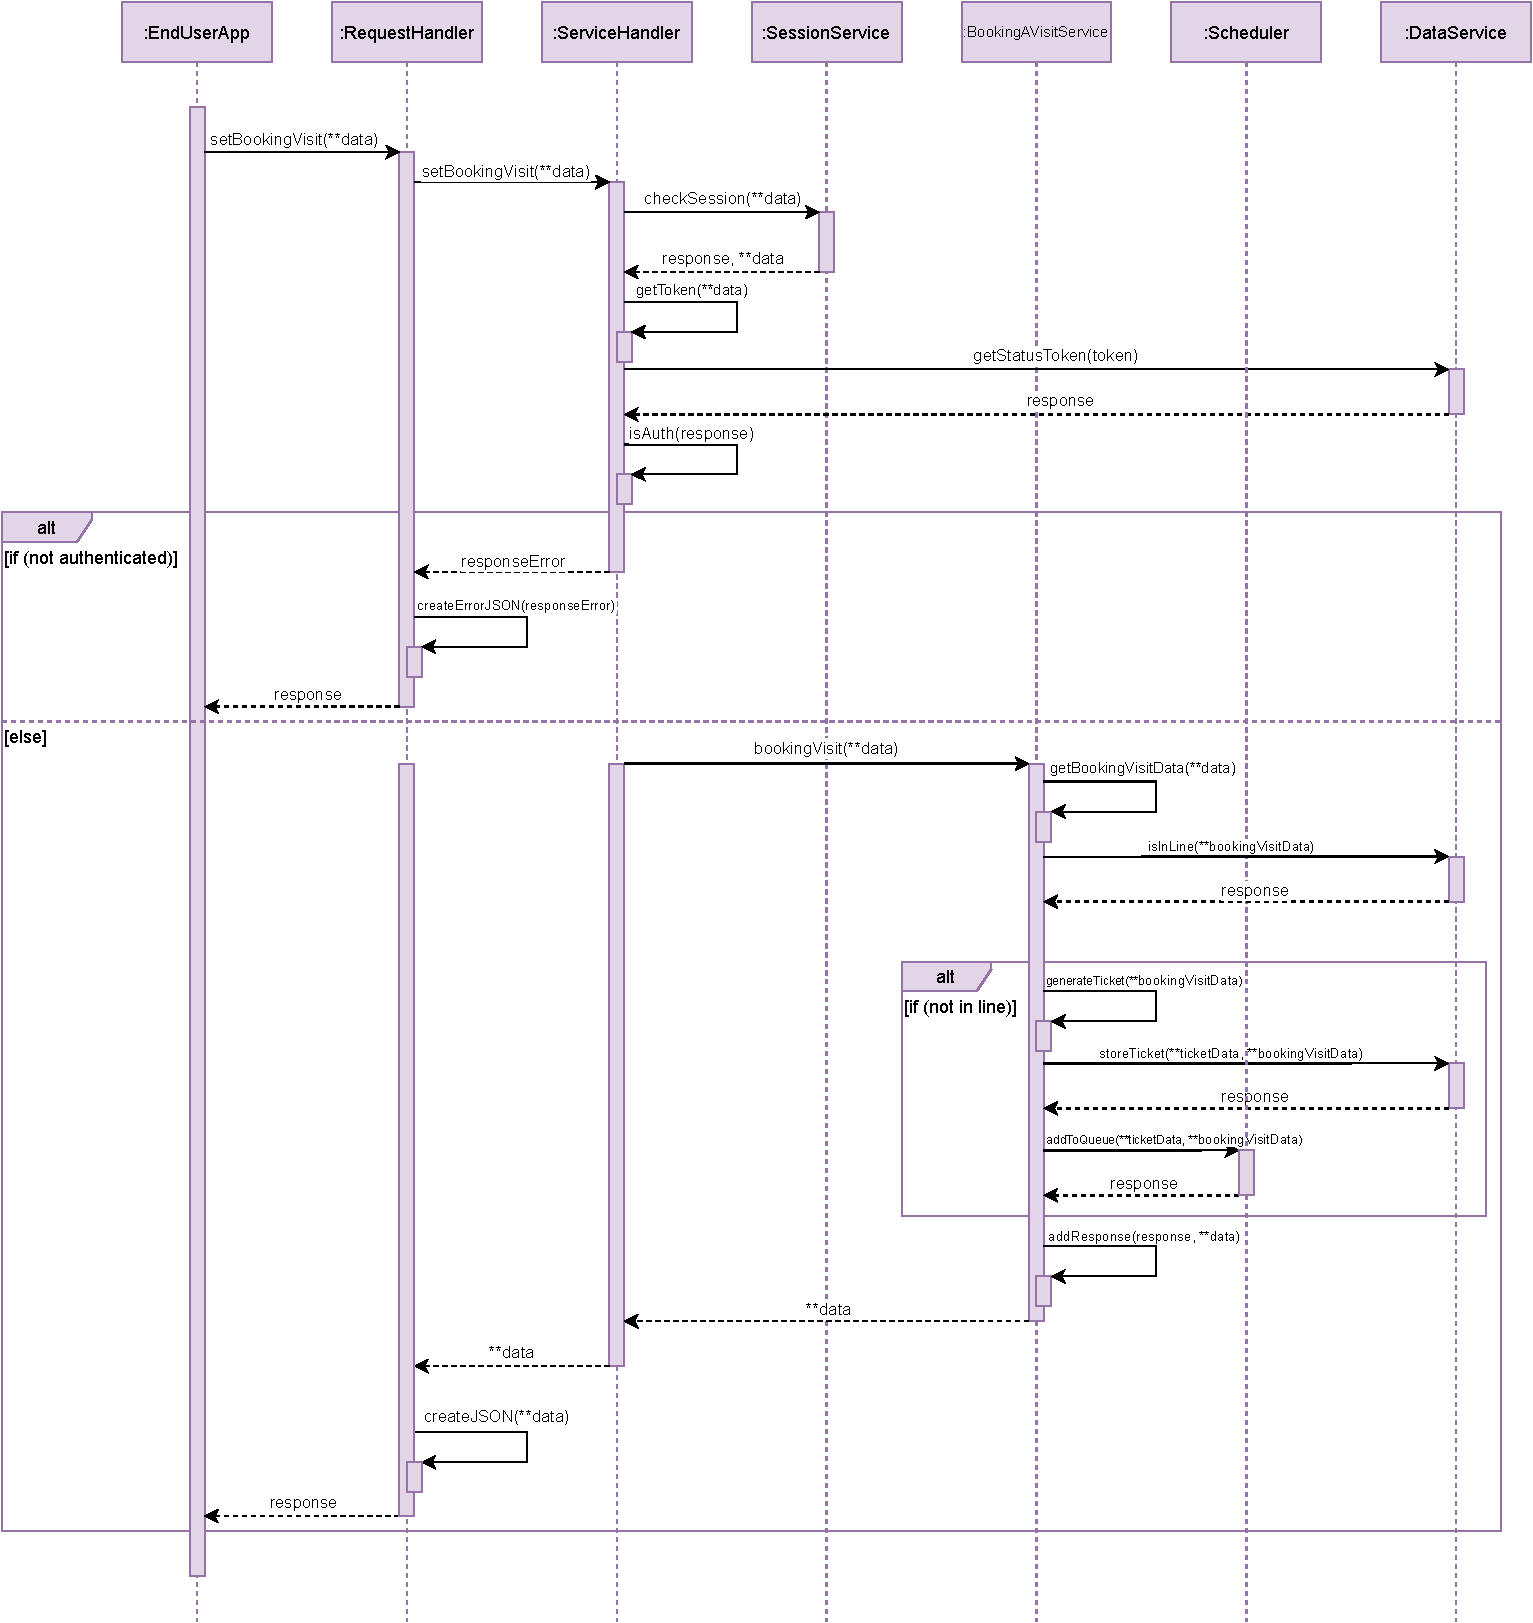
\includegraphics[width=1.0\textwidth]{images/bookingVisit_sequence_diagram.pdf}
	\caption{Booking a Visit sequence diagram.}\label{fig:BookingVisit}
\end{figure}

\subsection{Static Scheduler}

Figure~\ref{fig:StaticScheduler} illustrates the sequence of events that occur in the Scheduler after that the LiningUpService, or BookingAVisitService, has been activated.
It is called \textit{static} since these operations are performed only one time.
The main purpose of this sequence is to show how the system allocates tickets in the virtual queue. It estimates the time in which customers will be called by collecting data from the history of purchases of customers (GroceryStoreService) and the needed time to arrive to the store (GoogleMapsService). Once an estimation is computed, the allocation in the queue is determined.

\begin{figure}[H]
	\centering
	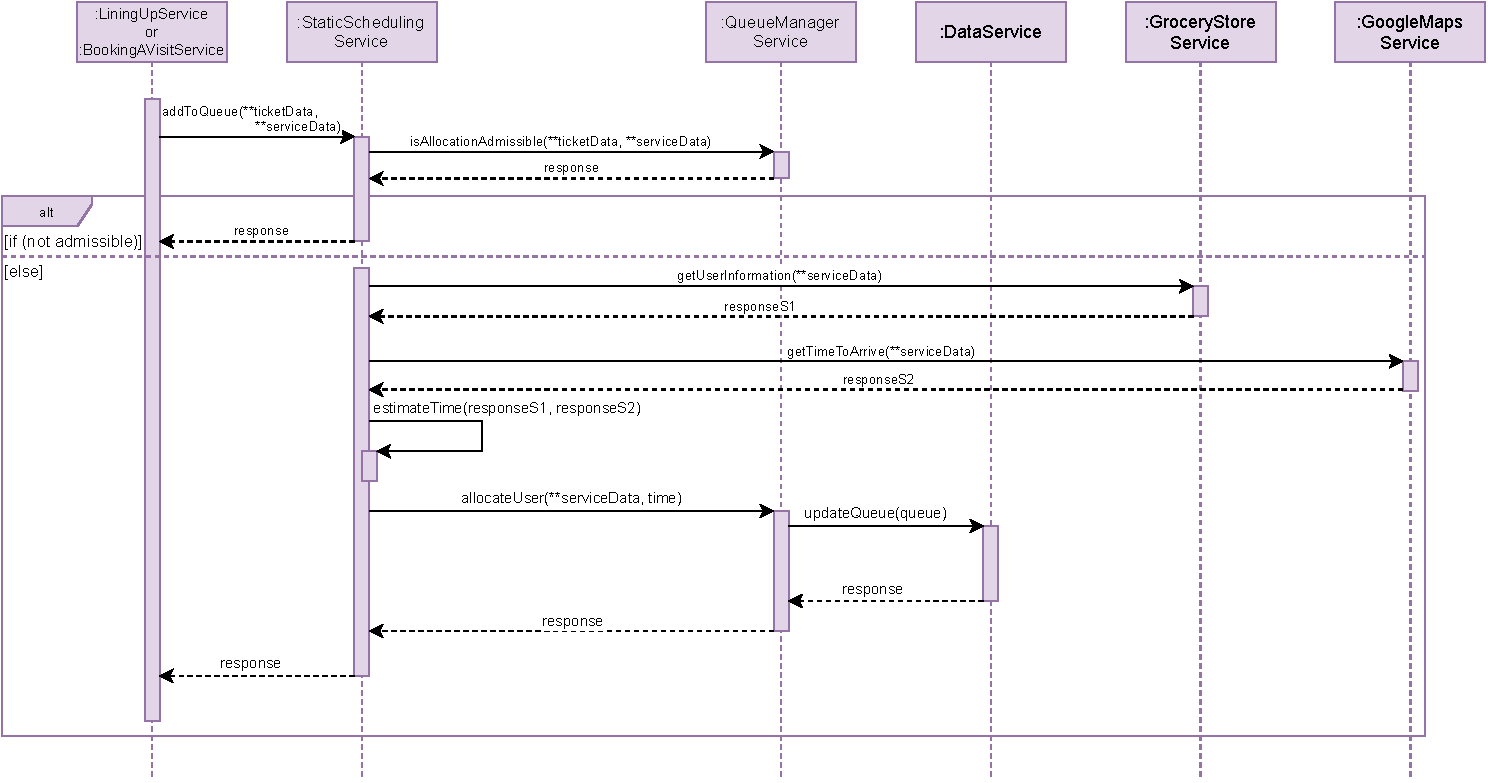
\includegraphics[width=1.0\textwidth]{images/scheduler_sequence_diagram.pdf}
	\caption{Static Scheduler sequence diagram.}\label{fig:StaticScheduler}
\end{figure}

\subsection{Dynamic Scheduler}

In contrast to the previous paragraph, in figure~\ref{fig:DynamicScheduler} there are activities that are performed mainly in background by the system to reschedule the virtual queue and to notify customers; for this reason it is called \textit{dynamic}.
The EndUserApp periodically sends information to the server about the location of the customers (in case of active tickets). These kind of requests are forwarded to the UserPositionService through the LiningUpService, or the BookingAVisitService. The UserPositionService is used to estimate the time to arrive of customers and to update the queue through the QueueManagerService.
The QueueManagerService checks if it should notify users about timing and delays, moreover it updates the queue if tickets are expired.

\begin{figure}[H]
	\centering
	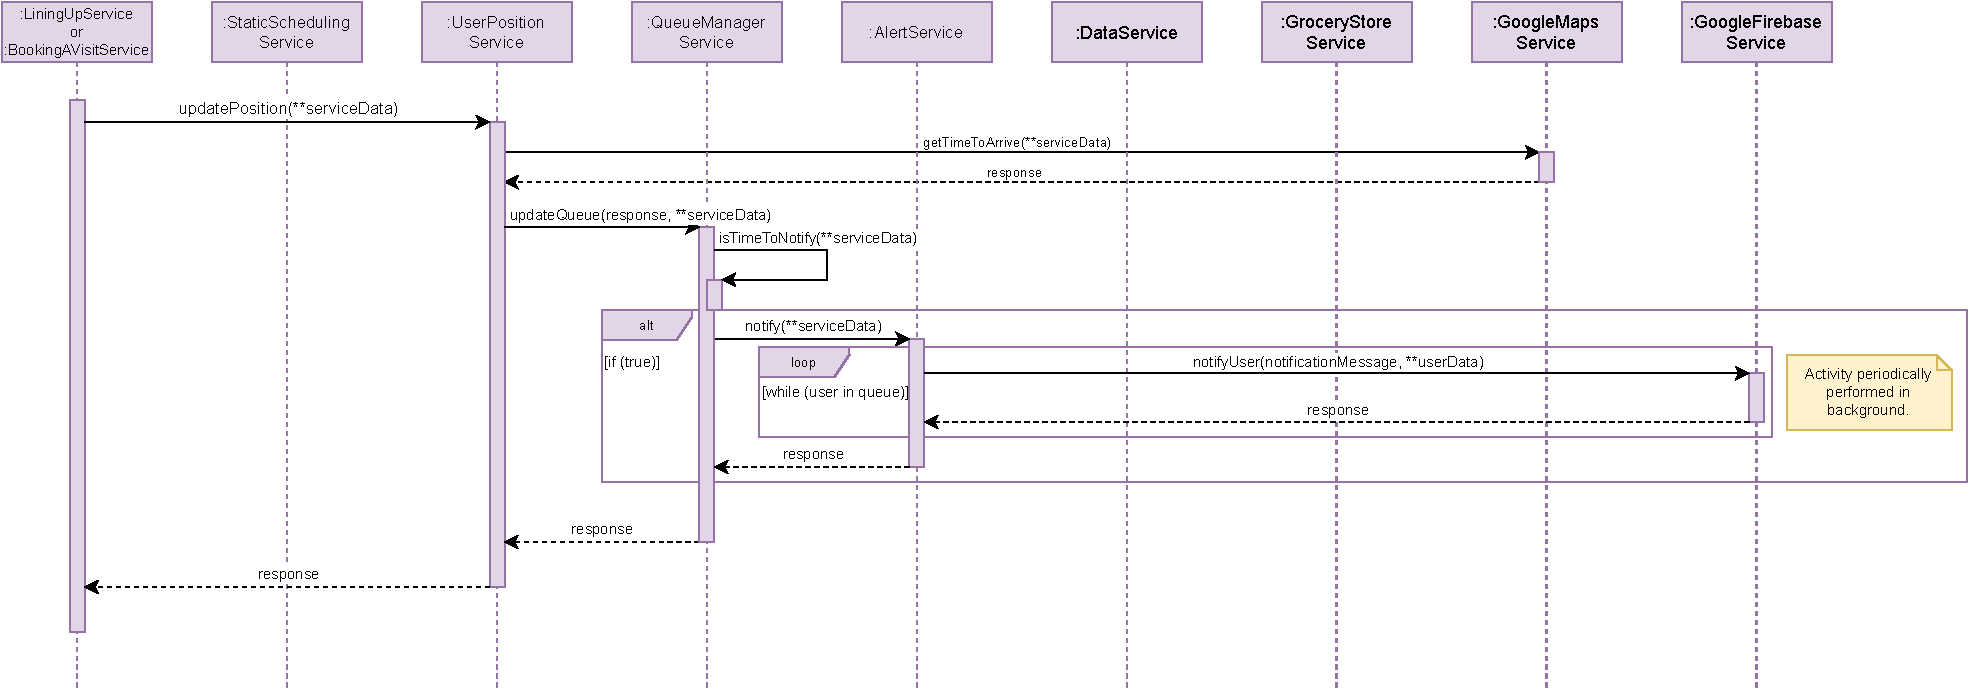
\includegraphics[width=1.0\textwidth]{images/dynamicScheduler_sequence_diagram.pdf}
	\caption{Dynamic Scheduler sequence diagram.}\label{fig:DynamicScheduler}
\end{figure}

\subsection{Control Queue}

This service is used by the store manager to modify the parameters of the scheduler algorithm.
Figure~\ref{fig:ControlQueue} follows the sequence of events to achieve this task. Since this operation can be activated only by store managers, the ControlQueueService verifies that the request is coming from a store manager account. In case of positive response, it will continue with a sequence of activities to update the parameters of the algorithm.

\begin{figure}[H]
	\centering
	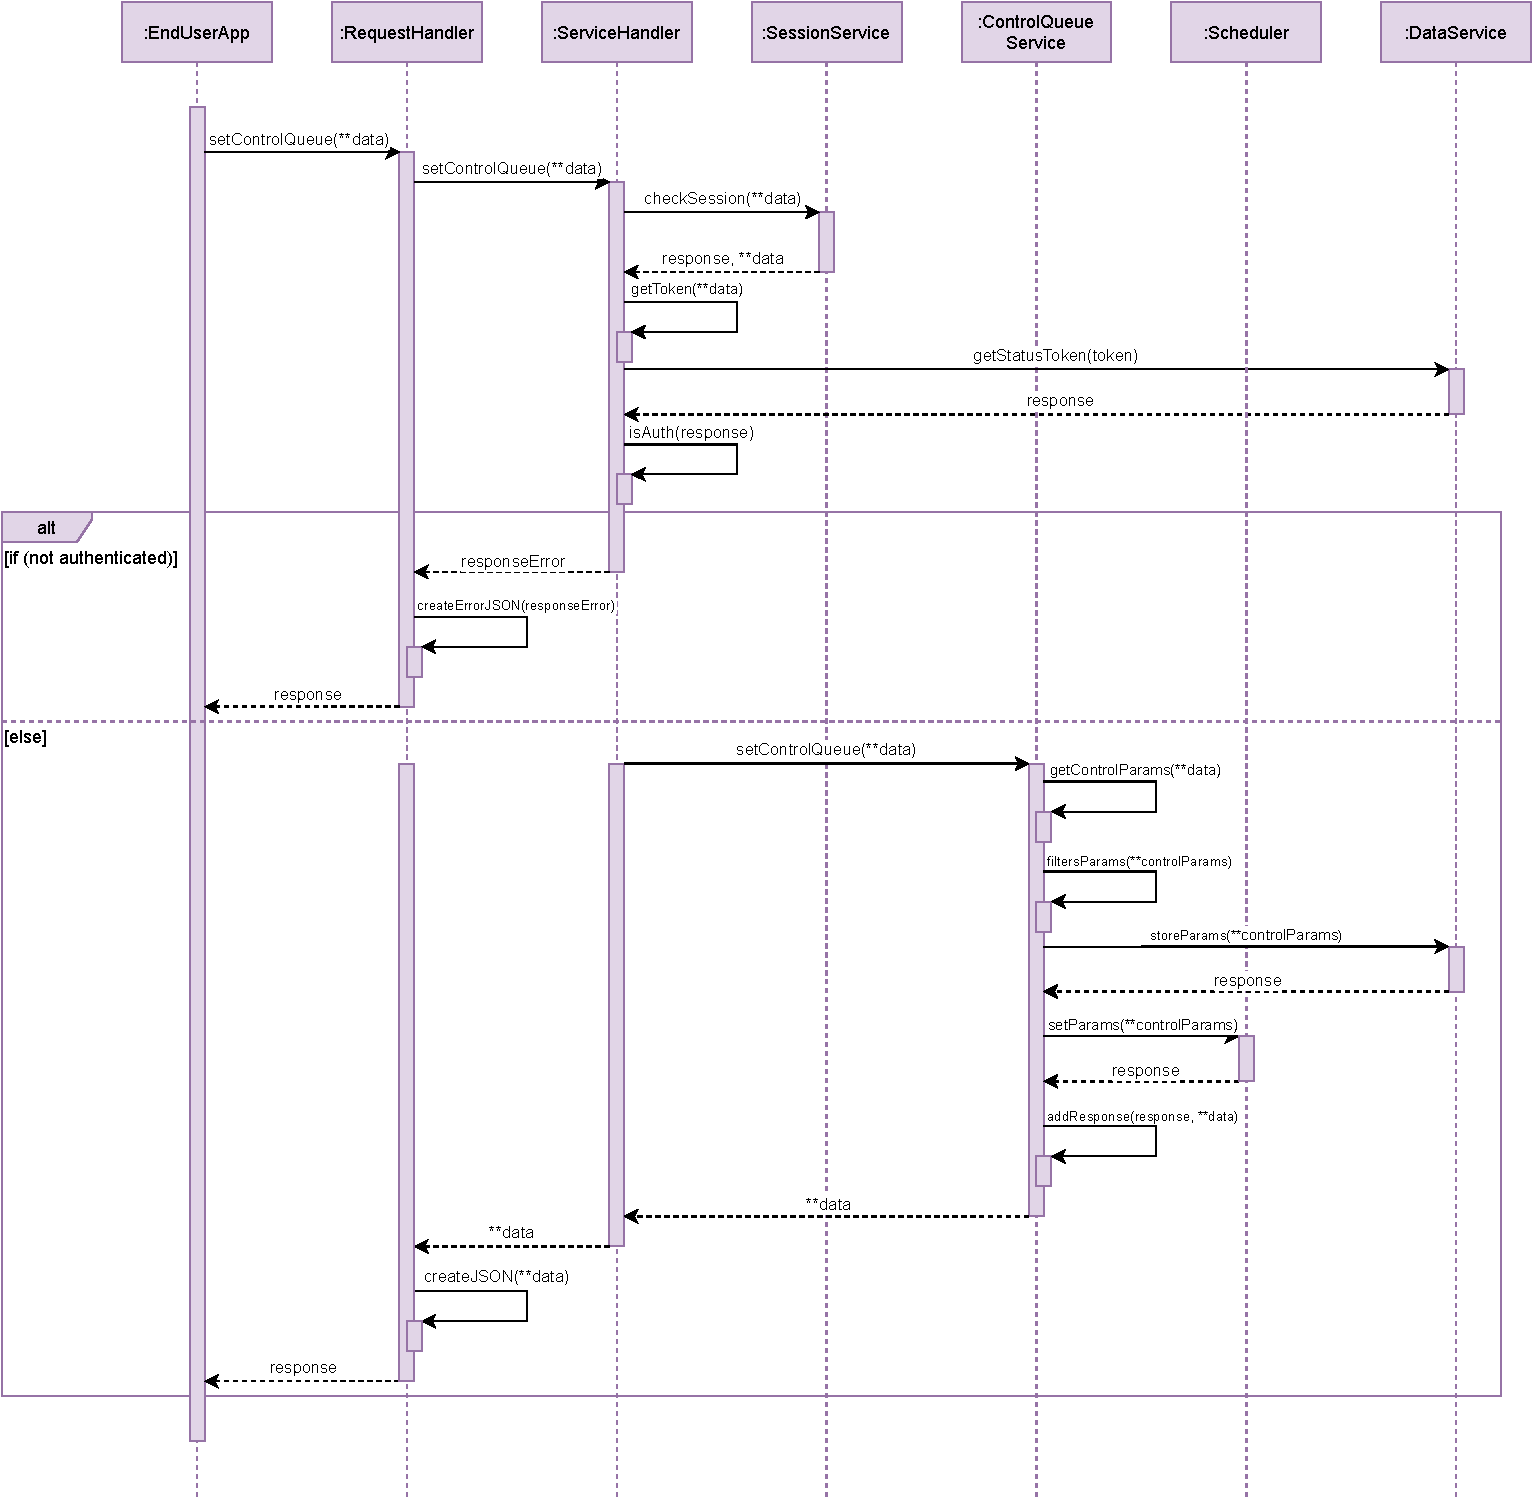
\includegraphics[width=1.0\textwidth]{images/controlQueue_sequence_diagram.pdf}
	\caption{Control Queue sequence diagram.}\label{fig:ControlQueue}
\end{figure}

\subsection{Show Stats}

Similarly to the previous paragraph, figure~\ref{fig:ShowStats} shows how the server retrieves data for analytical purposes. As before, this is an activity allowed only by store managers.

\begin{figure}[H]
	\centering
	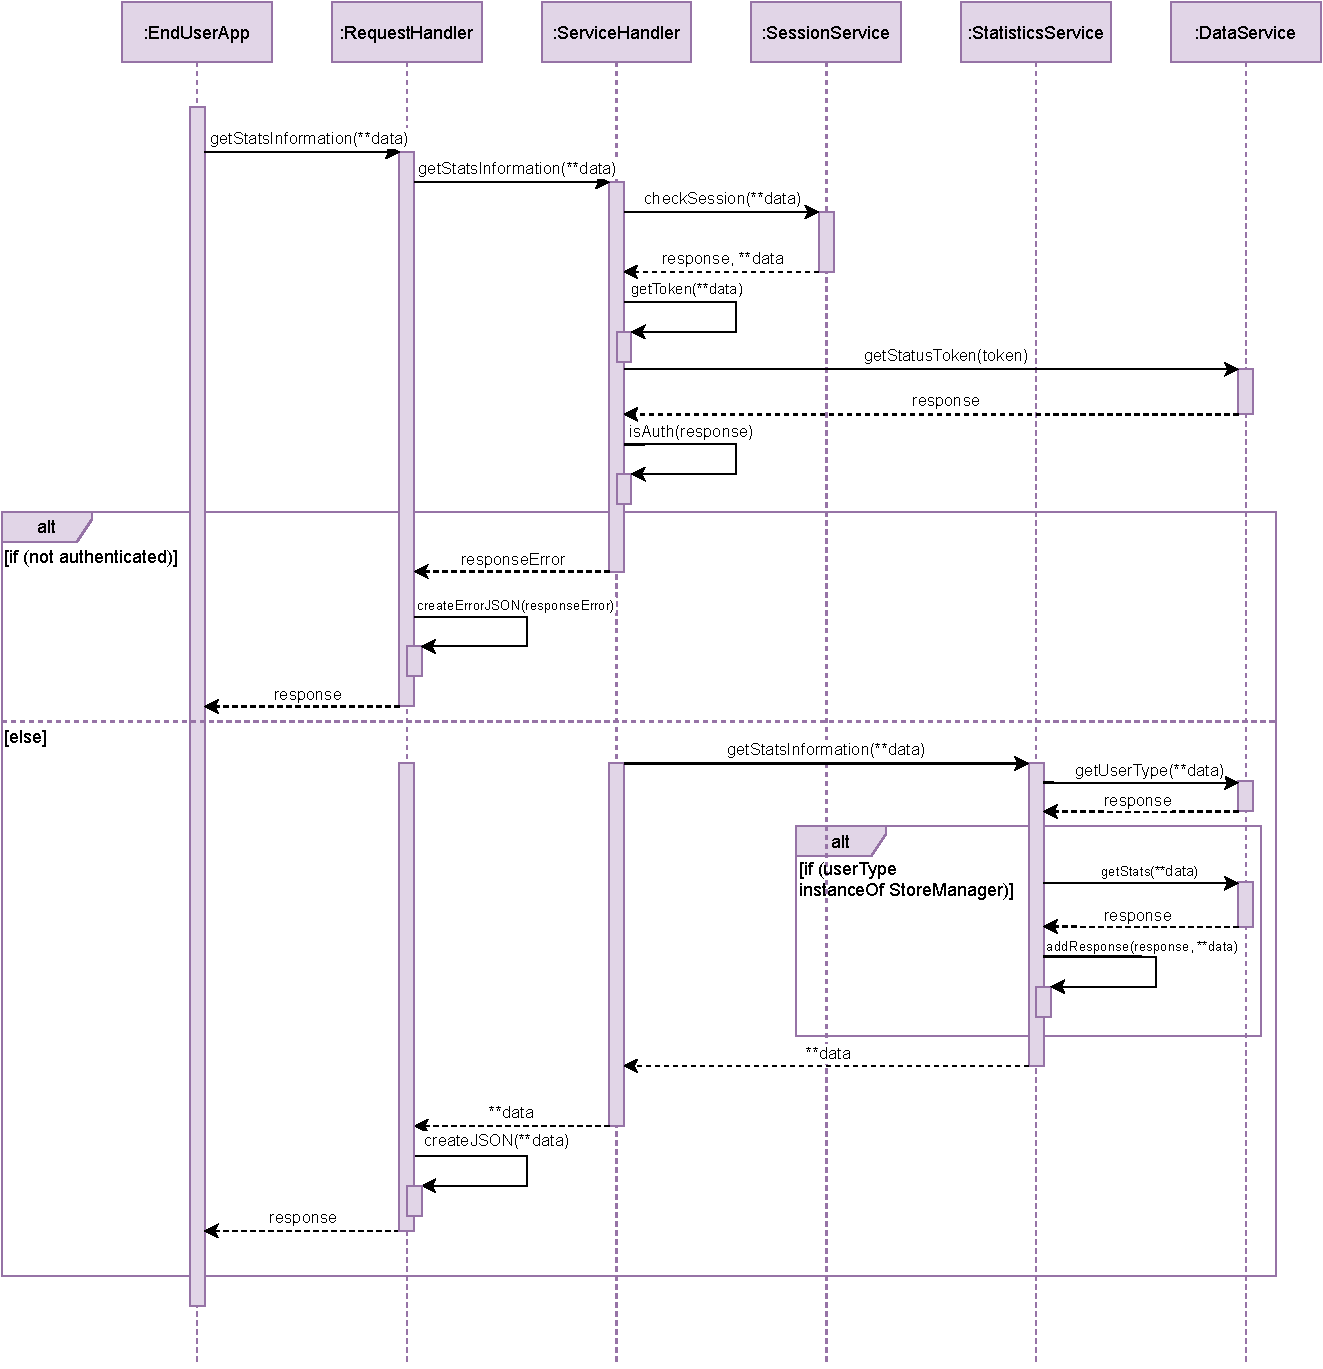
\includegraphics[width=1.0\textwidth]{images/showStats_sequence_diagram.pdf}
	\caption{Show Stats sequence diagram.}\label{fig:ShowStats}
\end{figure}

\subsection{QR Code Checking}

When customers scan the QR codes, the device of the store manager, in background, communicates with the server to authorize customers to enter in the store. Therefore, figure~\ref{fig:QRCodeChecking} reports the actions performed by the system to check that the scanned QR code is the same that has been called by the system.
This sequence diagram is strongly related to the corresponding one reported in the \gls{rasd}.

After having scanned the QR code, the EndUserApp of the store manager sends the ticket number to the server that compares it with the expected number.
If it is the same, the server reply to the EndUserApp that unlocks the turnstile and sends a confirmation to the server that save and update the status of the queue.

This is an activity that can be executed only by the store manager account, thus a verification must be performed as in figures~\ref{fig:ControlQueue} and \ref{fig:ShowStats} on the entity type. In this sequence, that verification wasn't be reported to avoid an overly crowded image.

\begin{figure}[H]
	\centering
	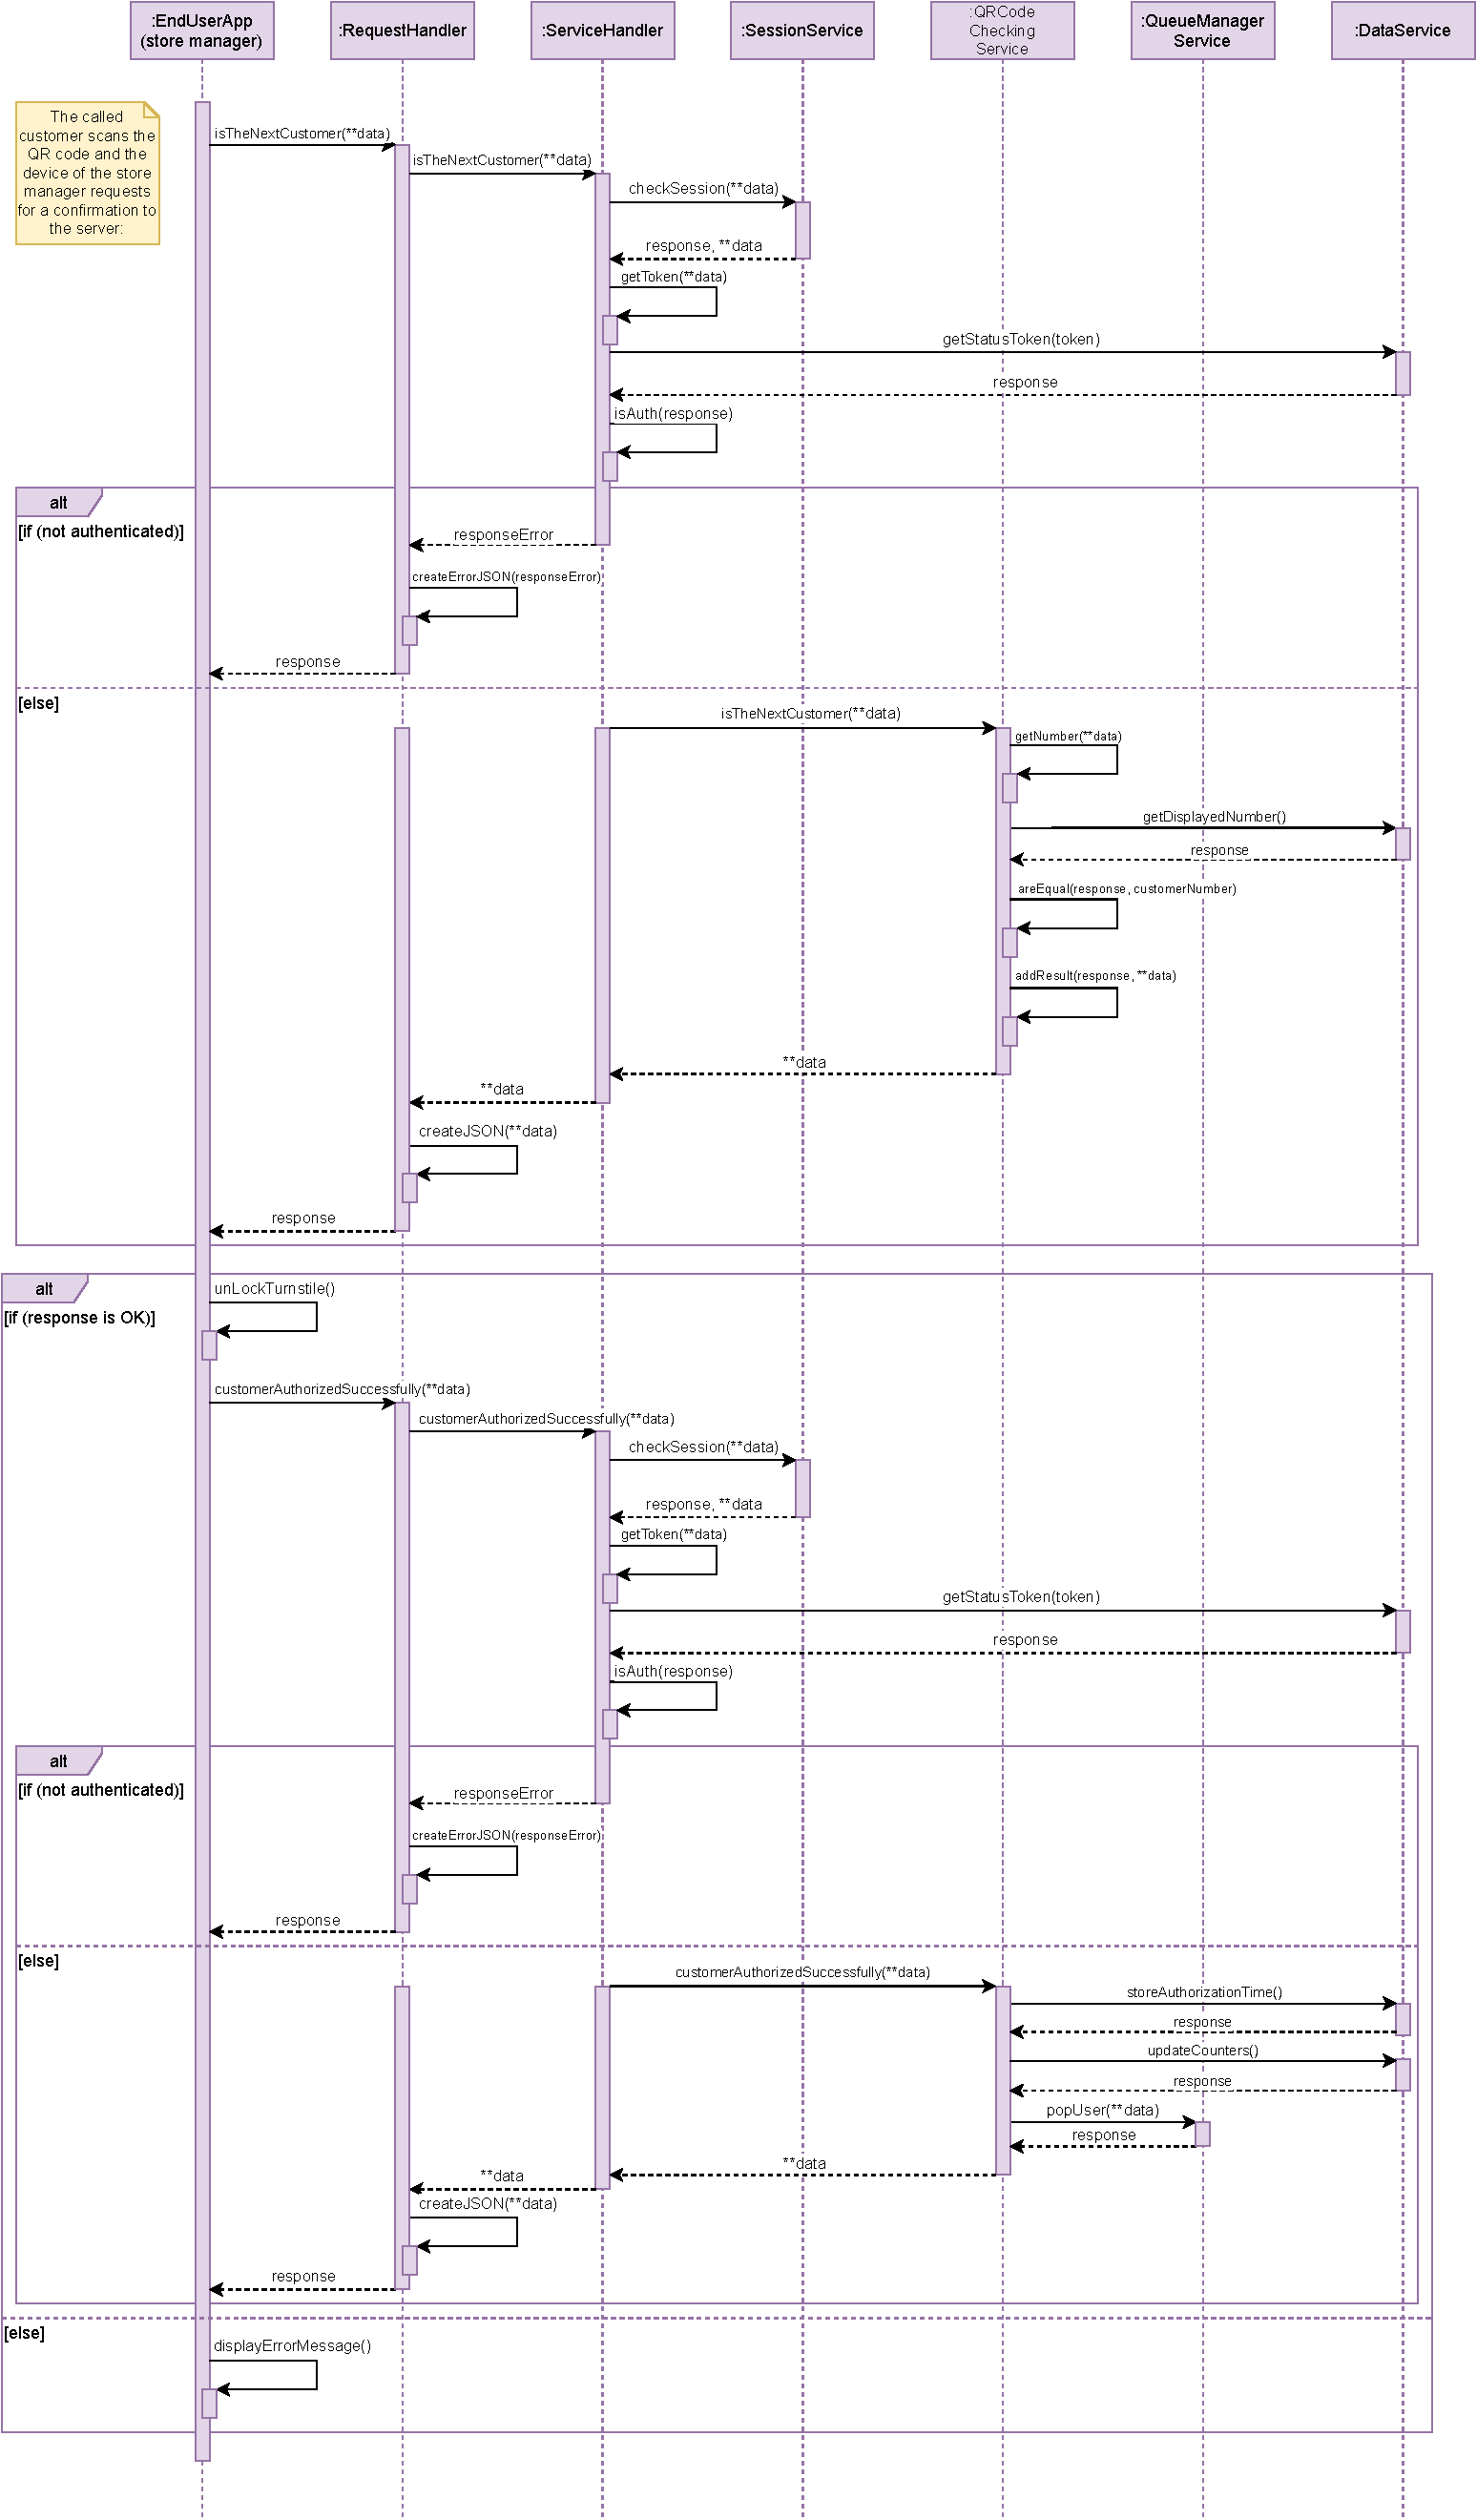
\includegraphics[width=0.8\textwidth]{images/qrCodeChecking_sequence_diagram.pdf}
	\caption{QR Code Checking sequence diagram.}\label{fig:QRCodeChecking}
\end{figure}

\section{Component Interfaces}
In this section, it is proposed a diagram that shows the different interface and the method used. It also shows which of them may interact during different operations. \\
The methods here shown are not supposed to be final but to give a hint of their function and suggest a possible way to implement them. 
\begin{figure}[H]
	\centering
	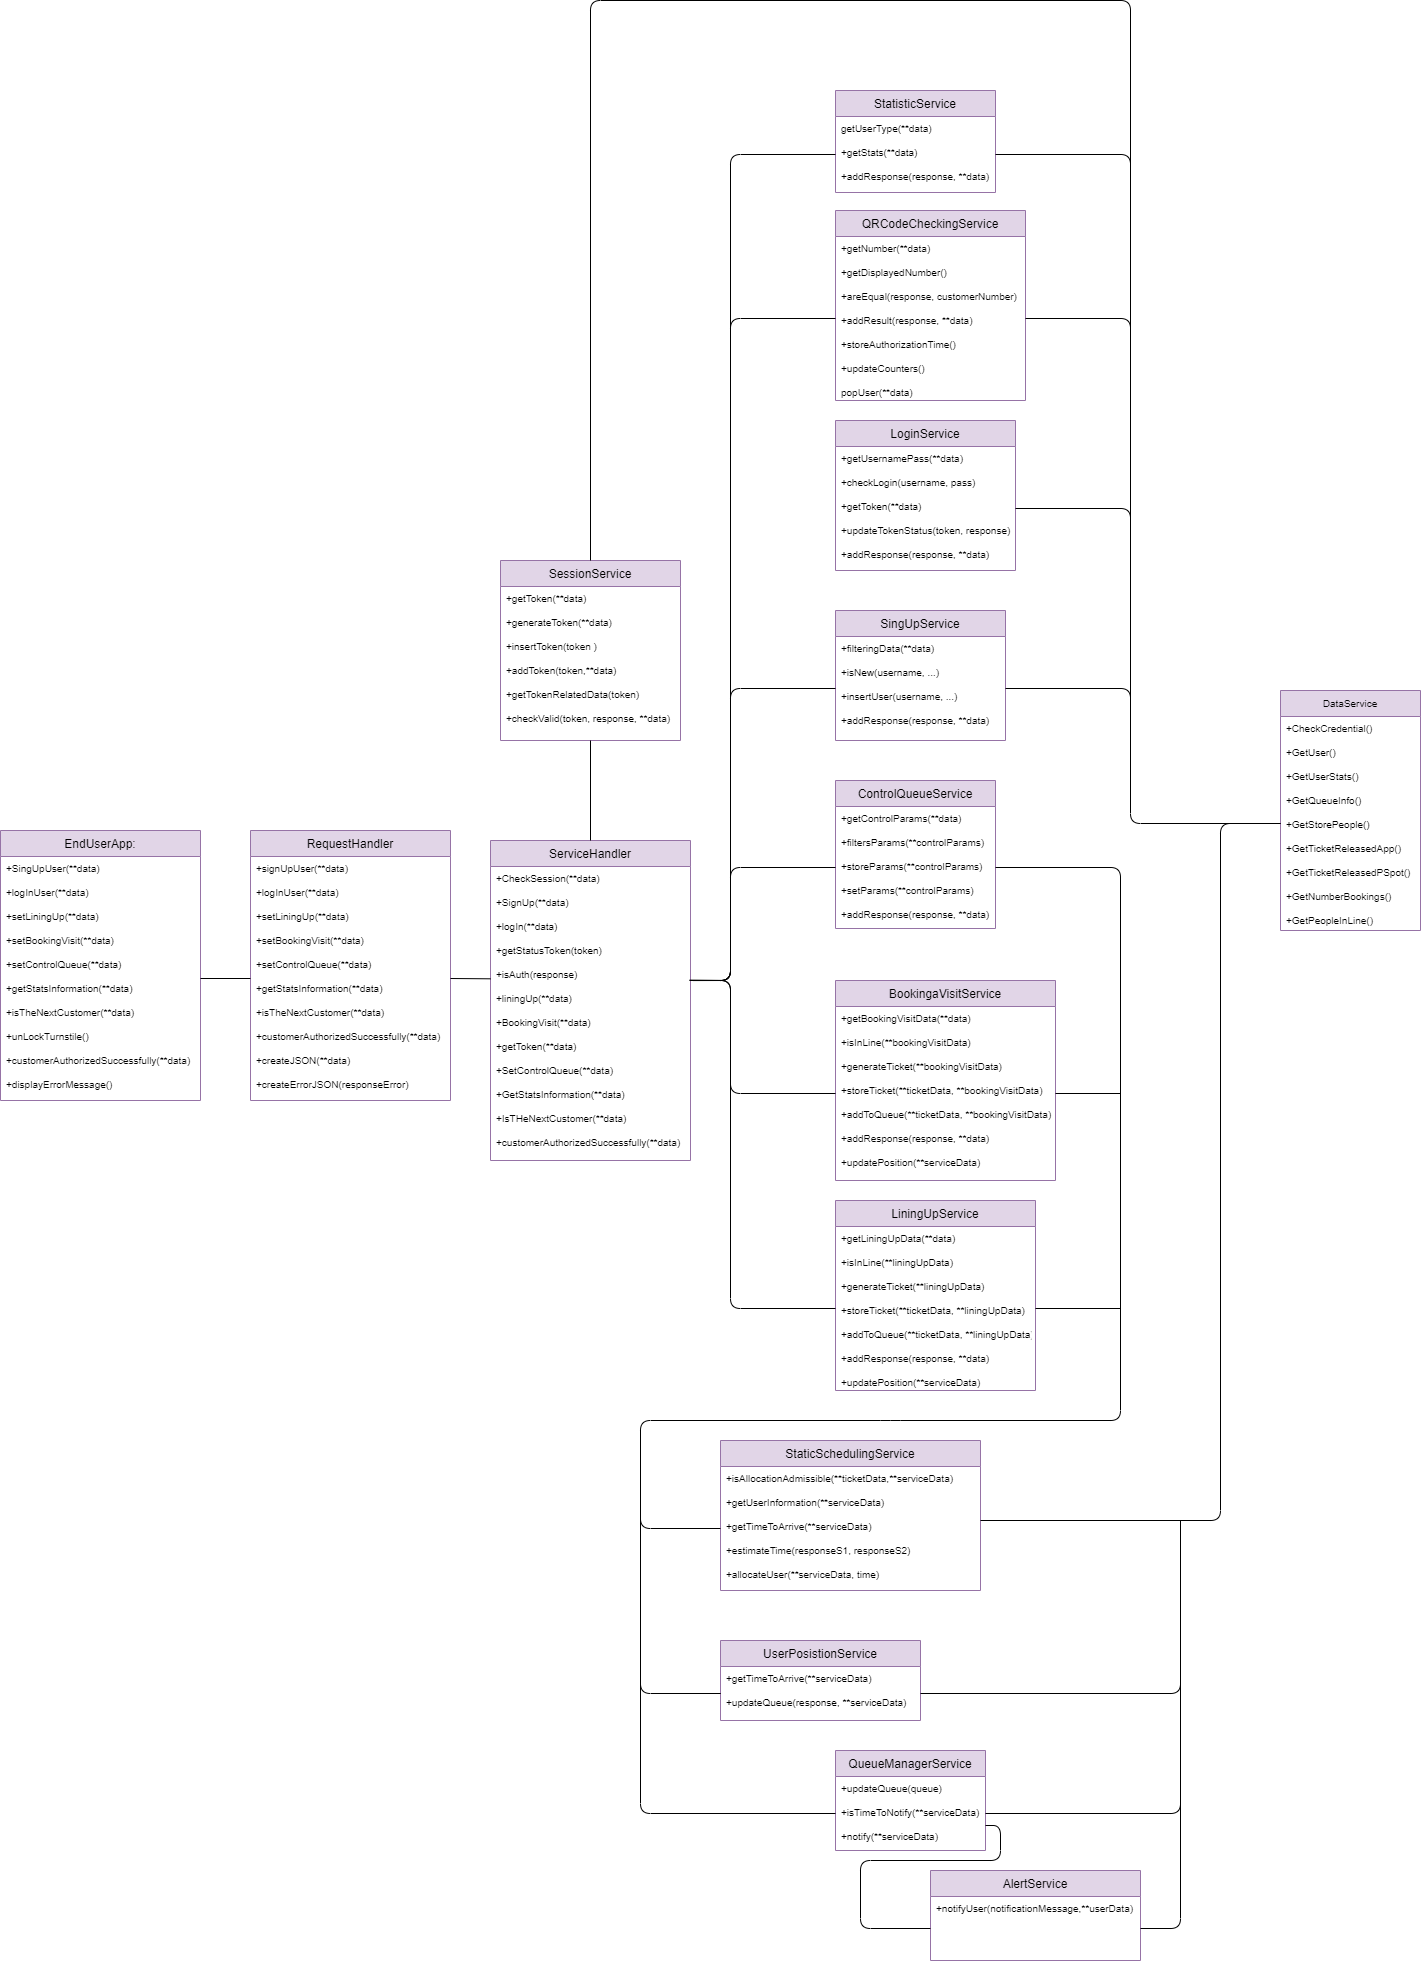
\includegraphics[width=1.0\textwidth]{images/Component_class_diagram.png}
	\caption{Component interface diagram.}\label{fig:Component interface diagram}
\end{figure}

\section{Selected Architectural Styles and Patterns}

\begin{figure}[H] % \begin{sidewaysfigure}
	\centering
	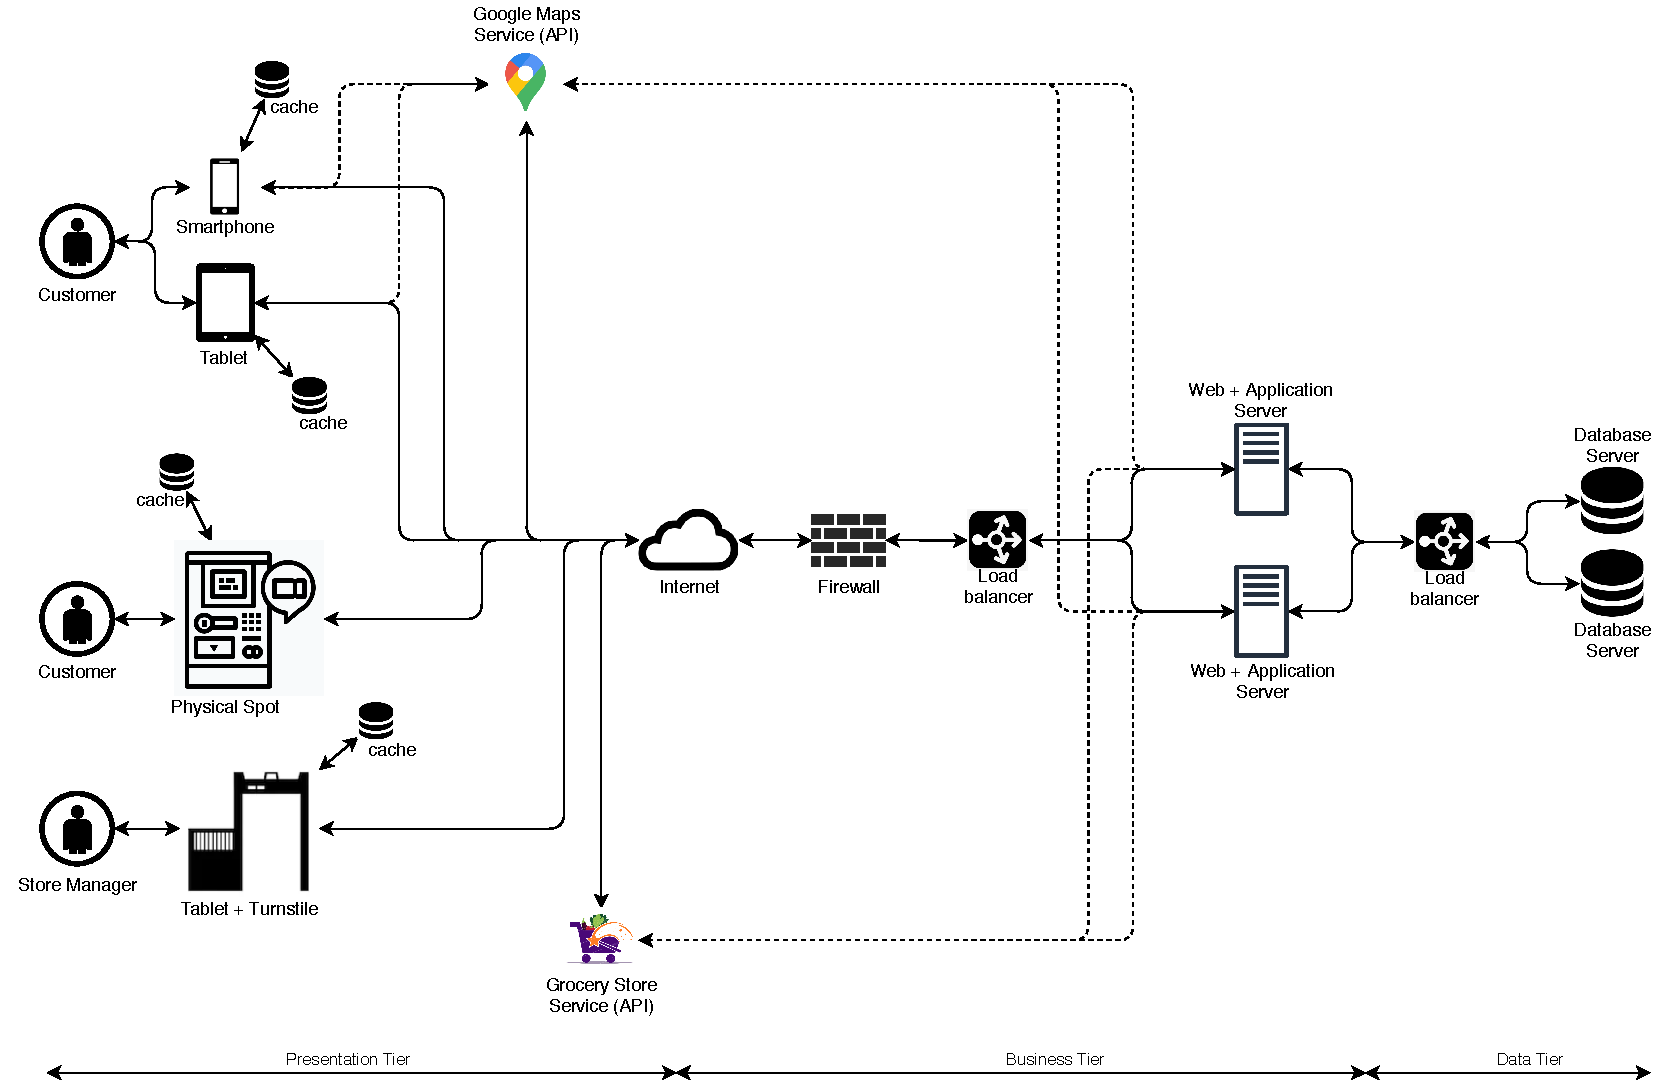
\includegraphics[width=1.0\textwidth]{images/architecture_components.pdf}
	\caption{Architecture components.}
\end{figure} % \end{sidewaysfigure}

\section{Other Design Decisions}